\documentclass[a4paper,12pt]{article}
\usepackage[utf8]{inputenc}
\usepackage[T1]{fontenc}
\usepackage{geometry}
\geometry{margin=1in}
\usepackage{booktabs}
\usepackage{amsmath}
\usepackage{graphicx}
\usepackage{caption}
\usepackage{subcaption}
\usepackage{longtable}
\usepackage{float}
\usepackage{hyperref}
\usepackage{colortbl}
\usepackage{xcolor}
\definecolor{lightgray}{RGB}{230,230,230}
\definecolor{red}{RGB}{255,107,107}
\definecolor{teal}{RGB}{78,205,196}
\definecolor{blue}{RGB}{69,183,209}
\definecolor{green}{RGB}{150,206,180}

% Preamble for tables and figures
\usepackage{booktabs}
\usepackage{array}
\usepackage{multirow}

% Font setup (last in preamble)
\usepackage{times} % Reliable serif font

\begin{document}

\title{MSDS-555: Project 04 \\ Customer Segmentation for Retail Strategy}
\author{Firoj Husen Shaikh}
\date{July 2025}
\maketitle

\section{Introduction}

This report details the comprehensive process and findings of a customer segmentation project utilizing the Online Retail dataset from the UCI Machine Learning Repository. The project aimed to leverage unsupervised learning techniques, specifically RFM (Recency, Frequency, Monetary) analysis and clustering, to segment customers into actionable groups. These segments enable targeted marketing strategies to enhance customer retention, boost engagement, and inform product recommendations, aligning with the strategic goals of a UK-based online retail store.

\section{Objective}

The key objectives of this project were:
\begin{itemize}
    \item Perform customer segmentation using RFM analysis to quantify purchasing behavior.
    \item Apply K-Means and Hierarchical clustering to identify distinct customer groups.
    \item Define actionable segments including loyal customers, at-risk customers, occasional buyers, and new customers.
    \item Provide data-driven marketing recommendations to improve retention and revenue.
\end{itemize}

\section{Data Description}

The dataset, sourced from the UCI Machine Learning Repository, encompasses transactional data from 01/12/2010 to 09/12/2011 for a UK-based online retail business. It includes the following features:
\begin{itemize}
    \item \textbf{InvoiceNo}: A unique identifier for each transaction.
    \item \textbf{StockCode}: A product-specific identifier.
    \item \textbf{Description}: The name or description of the product.
    \item \textbf{Quantity}: The number of items purchased in a transaction.
    \item \textbf{InvoiceDate}: The date and time of the transaction.
    \item \textbf{UnitPrice}: The price per unit of the item.
    \item \textbf{CustomerID}: A unique identifier for each customer.
    \item \textbf{Country}: The country of the customer.
\end{itemize}
The initial dataset contained approximately 541,909 rows, providing a rich foundation for analysis.

\section{Data Cleaning}

To ensure data quality, the following cleaning steps were applied:
\begin{itemize}
    \item Removed rows with missing \textbf{CustomerID} values, as these are essential for customer-level analysis.
    \item Excluded cancelled orders, identified by \textbf{InvoiceNo} starting with 'C'.
    \item Removed transactions with negative or zero \textbf{Quantity} or \textbf{UnitPrice} to eliminate invalid entries.
    \item Created a new \textbf{TotalAmount} column by multiplying \textbf{Quantity} and \textbf{UnitPrice} to reflect transaction value.
    \item Filtered the dataset to include only customers from the United Kingdom for focused analysis.
\end{itemize}
These steps reduced the dataset from 541,909 rows to 329,807 rows, removing approximately 39% of the data due to missing values, cancellations, and non-UK transactions.

\section{RFM Analysis}

RFM analysis was conducted to quantify customer behavior based on three metrics:
\begin{itemize}
    \item \textbf{Recency}: The number of days since a customer's last purchase, calculated with a reference date of 10-Dec-2011 (one day after the last transaction).
    \item \textbf{Frequency}: The total number of unique invoices per customer, indicating purchase frequency.
    \item \textbf{Monetary}: The total revenue generated by a customer, derived from the sum of \textbf{TotalAmount}.
\end{itemize}
These metrics were computed for each customer and normalized using StandardScaler to prepare for clustering. Across the dataset, the average Recency was 91 days, Frequency was 5.1 invoices, and Monetary value was £2,052, reflecting a wide range of customer engagement levels.

\section{Clustering Techniques}

\subsection{K-Means Clustering}

The optimal number of clusters was determined using the Elbow Method, which identified k=4 as the point of diminishing returns in inertia reduction. This choice was validated with a Silhouette score of 0.42, indicating reasonable cluster separation. The resulting clusters, based on normalized RFM values, are detailed below, with a visual representation provided in Figure \ref{fig:kmeans_scatter}.

\begin{figure}[H]
    \centering
    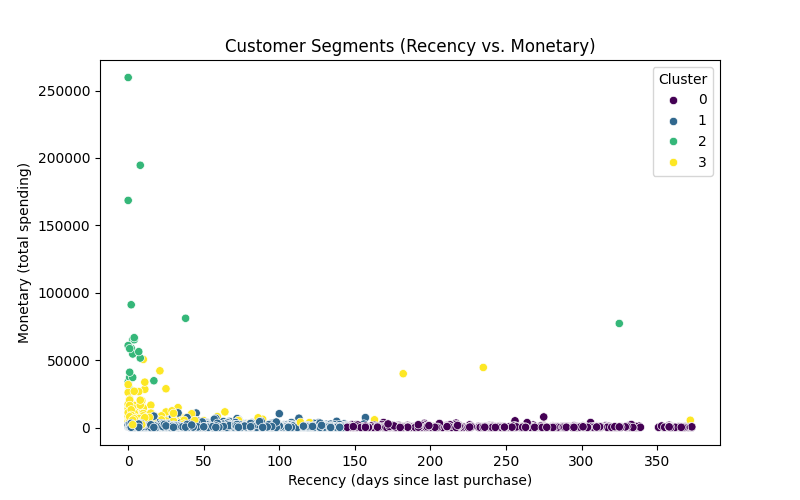
\includegraphics[width=0.8\textwidth]{kmeans_scatter.png}
    \caption{Scatter plot of Recency versus Monetary values, colored by K-Means cluster, illustrating the distinct separation of the four customer groups. Cluster 2 (Loyal Customers) is evident near low Recency and high Monetary values, while Cluster 0 (At-Risk Customers) appears at high Recency and low Monetary values.}
    \label{fig:kmeans_scatter}
\end{figure}

The clusters are:
\begin{itemize}
    \item \textbf{Cluster 0}: Average Recency 246.62 days, Frequency 1.56, Monetary £437.94, with 962 customers.
    \item \textbf{Cluster 1}: Average Recency 44.33 days, Frequency 3.33, Monetary £1,139.25, with 2,646 customers.
    \item \textbf{Cluster 2}: Average Recency 18.78 days, Frequency 59.91, Monetary £71,494.41, with 23 customers.
    \item \textbf{Cluster 3}: Average Recency 16.04 days, Frequency 17.17, Monetary £7,710.26, with 289 customers.
\end{itemize}

\subsection{Hierarchical Clustering}

Agglomerative Clustering with Ward linkage was applied, confirming k=4 clusters. A dendrogram, generated from a random subset of 50 customers, revealed four major branches at a distance threshold of approximately 6–8, aligning with the K-Means results. The hierarchical clustering process is visualized in Figure \ref{fig:dendrogram}, which supports the segmentation by showing hierarchical groupings.

\begin{figure}[H]
    \centering
    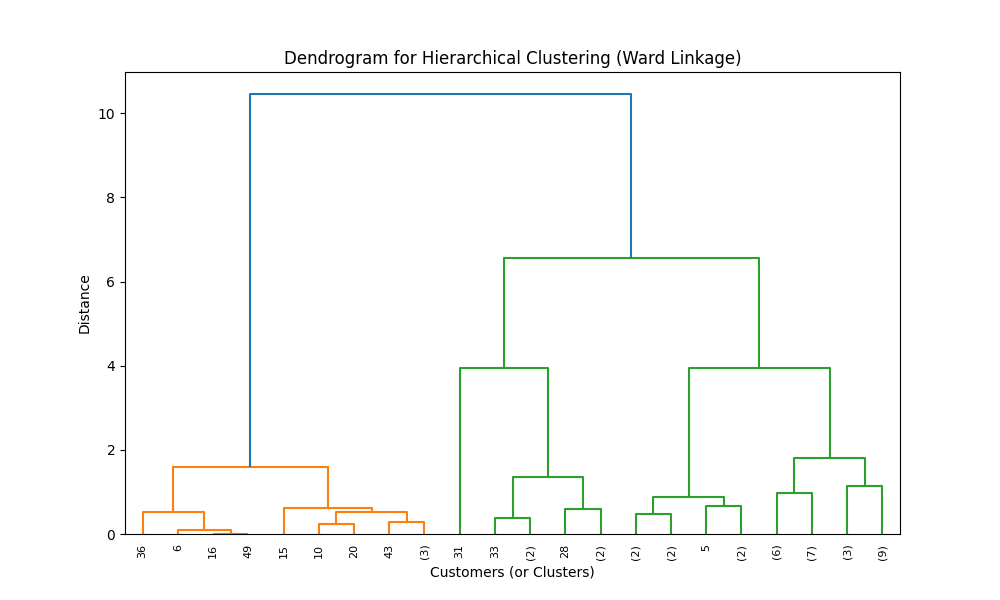
\includegraphics[width=0.8\textwidth]{dendrogram.png}
    \caption{Dendrogram for Hierarchical Clustering using Ward linkage, depicting the hierarchical merging of customers into four clusters. The tallest vertical line at around distance 10 indicates a primary split, with subsequent branches at lower distances confirming the four-group structure.}
    \label{fig:dendrogram}
\end{figure}

The hierarchical clusters exhibited similar RFM patterns to K-Means, validating the segmentation approach.

\section{Customer Segments Identified}

The clusters were mapped to actionable segments based on their RFM characteristics:
\begin{itemize}
    \item \textbf{Loyal Customers}: Characterized by low Recency (18.78 days), high Frequency (59.91), and high Monetary (£71,494.41), representing 23 highly engaged, high-value customers.
    \item \textbf{At-Risk Customers}: Marked by high Recency (246.62 days), low Frequency (1.56), and low Monetary (£437.94), including 962 customers at risk of churn.
    \item \textbf{Occasional Buyers}: Featuring moderate Recency (44.33 days), moderate Frequency (3.33), and moderate Monetary (£1,139.25), comprising 2,646 customers with sporadic purchases.
    \item \textbf{New Customers}: Defined by low Recency (16.04 days), moderate Frequency (17.17), and high Monetary (£7,710.26), consisting of 289 recently active customers.
\end{itemize}

\section{Recommendations}

Tailored marketing strategies for each segment include:
\begin{itemize}
    \item \textbf{Loyal Customers}: Offer loyalty rewards and exclusive deals to maintain their high engagement and spending.
    \item \textbf{At-Risk Customers}: Send win-back emails and personalized offers to re-engage these dormant customers.
    \item \textbf{Occasional Buyers}: Provide purchase reminders and discounts on related items to increase purchase frequency.
    \item \textbf{New Customers}: Extend welcome offers and guided onboarding to encourage repeat purchases and build loyalty.
\end{itemize}

\section{Dashboard Overview}

An interactive dashboard was developed using Streamlit to visualize the segmentation results. Key components include:

\begin{itemize}
    \item \textbf{RFM Distributions}: Histograms display the distribution of Recency, Frequency, and Monetary values across all customers. Figure \ref{fig:rfm_recency} shows the Recency distribution, Figure \ref{fig:rfm_frequency} the Frequency distribution, and Figure \ref{fig:rfm_monetary} the Monetary distribution, with colors red, teal, and blue respectively to distinguish each metric.

    \begin{figure}[H]
        \centering
        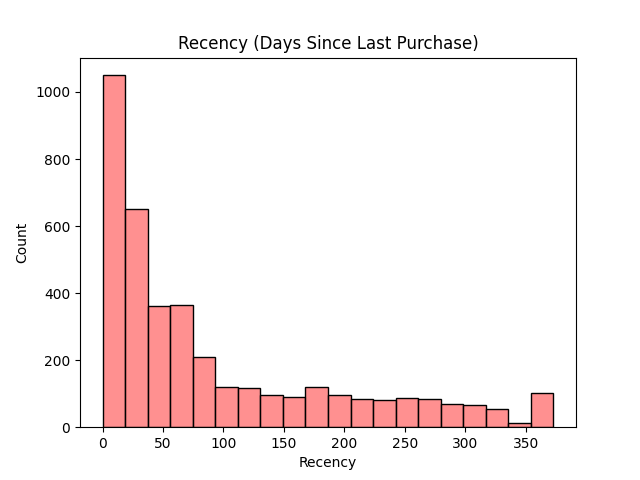
\includegraphics[width=0.8\textwidth]{rfm_dist_recency.png}
        \caption{Histogram of Recency distribution, highlighting the spread of days since last purchase, with a peak indicating a significant number of customers with moderate to high Recency.}
        \label{fig:rfm_recency}
    \end{figure}

    \begin{figure}[H]
        \centering
        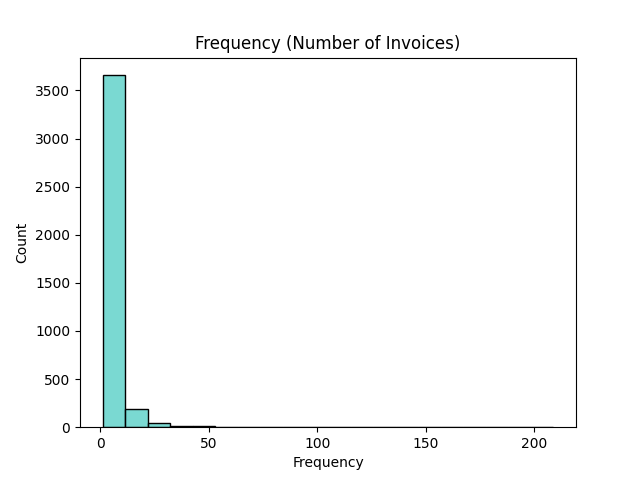
\includegraphics[width=0.8\textwidth]{rfm_dist_frequency.png}
        \caption{Histogram of Frequency distribution, showing the number of unique invoices per customer, with a skew towards lower frequencies.}
        \label{fig:rfm_frequency}
    \end{figure}

    \begin{figure}[H]
        \centering
        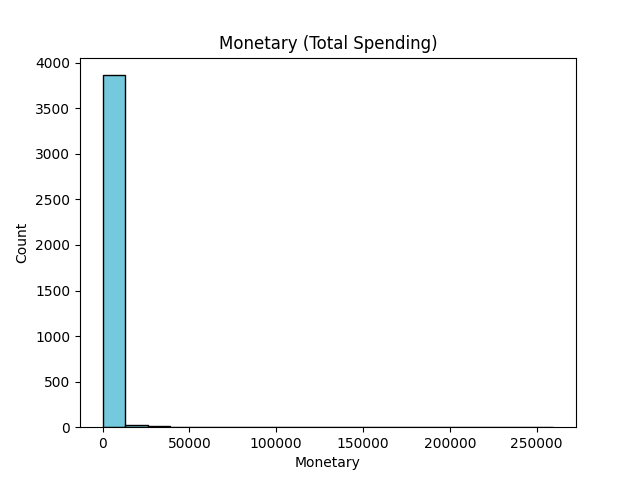
\includegraphics[width=0.8\textwidth]{rfm_dist_monetary.png}
        \caption{Histogram of Monetary distribution, illustrating total spending with a long tail due to high-value customers like those in the Loyal segment.}
        \label{fig:rfm_monetary}
    \end{figure}

    \item \textbf{Segment Sizes and Attributes}: A table presents the average Recency, Frequency, Monetary values, and customer counts for each segment, offering a concise overview.

    \item \textbf{Revenue by Segment}: A bar chart illustrates total revenue per segment, with Loyal Customers in red, At-Risk Customers in teal, Occasional Buyers in blue, and New Customers in green. Figure \ref{fig:revenue_segment} highlights the revenue dominance of Loyal Customers.

    \begin{figure}[H]
        \centering
        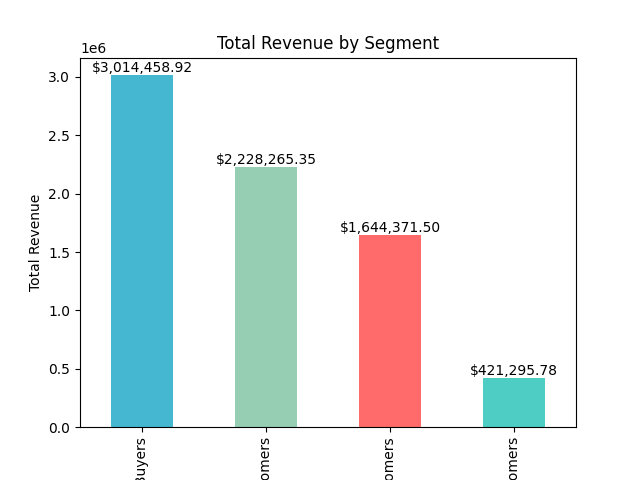
\includegraphics[width=0.8\textwidth]{revenue_by_segment.png}
        \caption{Bar chart of total revenue by segment, demonstrating that Loyal Customers contribute the highest revenue, followed by New Customers, with clear visual distinction using segment-specific colors.}
        \label{fig:revenue_segment}
    \end{figure}

    \item \textbf{Marketing Recommendations}: Textual guidance provides actionable strategies for each segment.
\end{itemize}

To include these plots, save them from the Streamlit dashboard using `plt.savefig('filename.png')` in the dashboard code, ensuring they are placed in the same directory as this LaTeX file before compilation.

\section{Conclusion}

This project successfully identified and validated four meaningful customer segments through RFM analysis, K-Means clustering, and Hierarchical clustering. The segmentation strategy, supported by a Silhouette score of 0.42 and dendrogram validation, provides a robust foundation for targeted marketing. The interactive Streamlit dashboard enhances accessibility, enabling stakeholders to explore insights and implement personalized engagement strategies to improve customer retention and increase revenue. The inclusion of visual diagrams further solidifies the analytical rigor, offering a clear representation of the clustering process and segmentation outcomes.

\begin{thebibliography}{9}
\bibitem{dataset} UCI Machine Learning Repository, Online Retail Dataset, \url{https://archive.ics.uci.edu/ml/datasets/Online+Retail}
\end{thebibliography}

\appendix
\section{Appendix}

\begin{itemize}
    \item \textbf{Codebase}: Jupyter Notebook and Python scripts available here \url{https://github.com/FirojShaikh/customer-segmentation-analysis}.
    \item \textbf{Dataset}: UCI Online Retail dataset.
    \item \textbf{Tools}: Python libraries including pandas, scikit-learn, matplotlib, seaborn, and Streamlit.
\end{itemize}

\end{document}